\documentclass[10pt,twoside,english,a4paper]{article}

\usepackage[english]{babel}
%\usepackage[T1]{fontenc}
\usepackage[IL2]{fontenc} % lepšia sadzba písmena Ľ než v T1
\usepackage[utf8]{inputenc}
\usepackage{graphicx}
\usepackage{subcaption}
\usepackage{url} % príkaz \url na formátovanie URL
\usepackage{hyperref} % odkazy v texte budú aktívne (pri niektorých triedach dokumentov spôsobuje posun textu)
\usepackage{float}
\usepackage{wrapfig}
\usepackage{mathtools}
\usepackage{cite}
%\usepackage{times}

\usepackage{geometry}
\geometry{top=1in, bottom=1in, left=1.5in, right=1.5in}

\pagestyle{headings}

\title{Recommendation systems for personalized advertising in digital marketing} % meno a priezvisko vyučujúceho na cvičeniach


\author{Vsevolod Salik\\[2pt]
	{\small Slovak University of Technology in Bratislava }\\
	{\small Faculty of Informatics and Information Technologies }\\
	{\small \texttt{xsalik@stuba.sk}}
	}

\date{\small 26. september 2024}



\begin{document}


\maketitle
\thanks{Semestral project in the subject Methods of engineering work, academic year 2024/25, supervised by Pavol Batalik}
%insert thanks part in the title after i figure out how it works



\begin{abstract}
	In the modern era, internet is the biggest information source humanity could ever imagine.  However, this tool’s effectiveness can be limited due to the lack of knowledge or accessibility of users. Recommendation systems help to assist users, by filtering information based on previous user interactions to create recommendations for them consisting of products relevant to their interests. Recommendation systems are used widely in various fields. This article will focus on covering personalized advertising in digital marketing field.
	%%todo end the second part of abstract based especially on digital marketing
\end{abstract}



\section{Introduction}
We live in a digital era, where technology plays an essential role in enhancing quality of life. Internet , one of the most transformative inventions, is the the largest repository of information ever created which can be used from almost every part of the world. Humanity gained an access to a such powerful tool which is beyond human capabilities, making it difficult to retain all the information encountered daily. That is the part where recommendation systems step in.

\medskip Recommendation systems provide information based on prior user interactions, tailored to match individual interests. They can be applied across various types of data, such as music, videos, articles, shopping, and services. This article focuses on personalized advertising in the field of digital marketing.

\medskip Competition on a marketplace grows daily. Targeting the appropriate audience and effectively selling products has become more complex comparing to previous years and that is why confronting a customer to make a purchase by simply showing them the advertisement is no longer effective enough.

\medskip The main focus of an advertising industry is not to send the ads to everyone but to find appropriate customers, who can be potentially interested in your product, afterward, create personalized advertisements, which will target them, to satisfy both customer needs and business financial objectives. Recommendation systems make it possible to identify relevant customers, tailoring content to each individual, recognizing preferences, and increasing their engagement. These are the primary functions of recommendation systems in digital marketing.

\medskip This article will briefly explore recommendation systems templates, describe principles of their work, examine the role of artificial intelligence, and present custom recommender engine implementations. The goal is to optimize the use of recommendation systems to create personalized advertising that increase sales efficiency.

%%\newpage

\section{Recommendation systems}
As shown on a figure \ref{fig:fig1}, model of an RS consists of user, item resource and recommendation algorithm \cite{8506344}.
Among these components, the recommendation algorithm is the most important part of RS\cite{ren2012research}\cite{zhang2015research}
The user model consists of computed preferences derived from personal data, including search history, purchase history, saved webpages, and so on.

Following this an item within the user’s field of interest is selected, and a recommendation is generated for presentation to the user.

The performance of a recommendation system is not covered in this section ,as it is directly related to the recommendation algorithm, which will be described in subsequent sections.

\begin{figure}[H]
	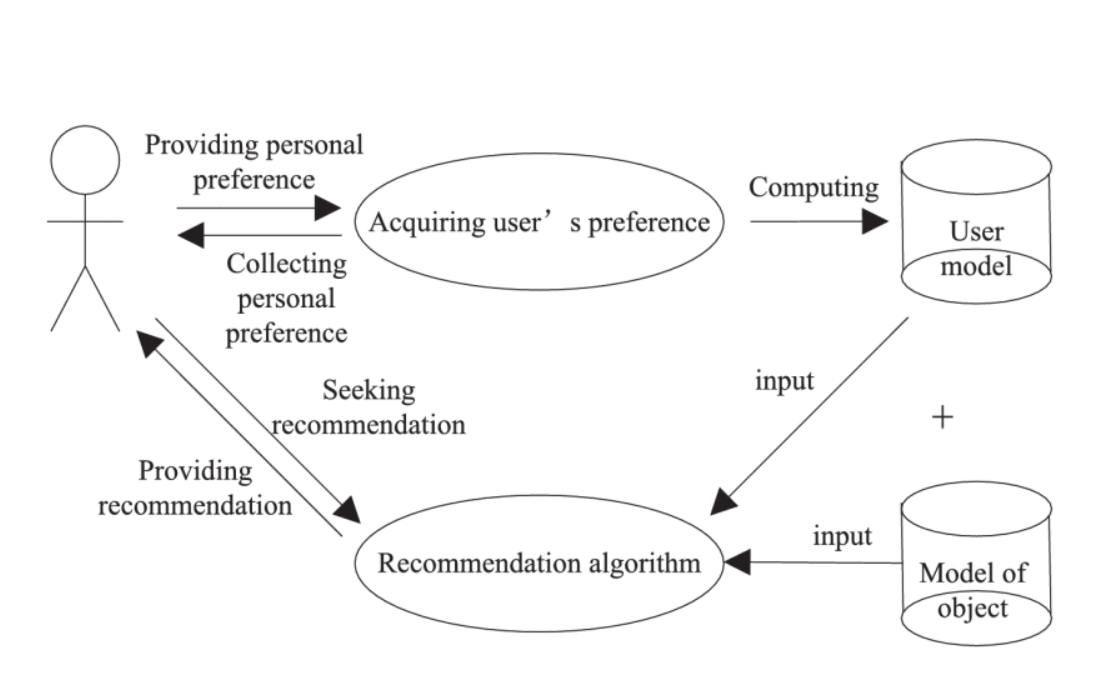
\includegraphics[width=1\textwidth]{./diagrams/recommender_system_model.png}
	\caption{Model of recommender systems. Reproduced from \cite{8506344}}
	\label{fig:fig1}
\end{figure}


\subsection{Types of recommender systems}

Different types of recommender systems serve distinct purposes. This article will focus on content-based methods, hybrid methods and primarly on to collaborative filtering methods.\ref{fig:fig2}
% bellow i am going to describe pros and cons of all the methods and try to find the most optimal one

\begin{figure}[H]
	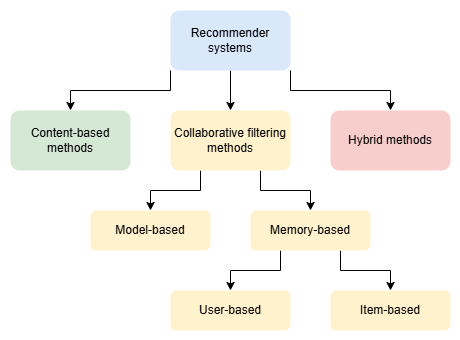
\includegraphics[width=1\textwidth]{./diagrams/recommender_systems_types.png}
	\caption{Types of recommender systems referenced in this article. Adapted from \cite{10113923}}
	\label{fig:fig2}
\end{figure}



%%\section{Trigger and triggered model}
%%Trigger and triggered model (TT) is an enhanced version of a recommendation system which provides anonymous recommendations, when user prioritizes privacy.



\section{Recommendation algorithms}

\subsection{Content-based}

In the vector space model user profiles can be represented just like documents by one 
or more profile vectors. The degree of similarity between a profile vector P, where 
P = ( \( u_1 \text{,...,} u_k \)) can be determined by using the cosine measure:\cite{LU228322}

\begin{equation*}\mathop{\text{sim}}\nolimits_{DP} = \frac{D \cdot P}{\|D\| \cdot \|P\|} = \frac{\sum\limits_k u_k \cdot w_k}{\sqrt{\sum\limits_k u_k^2 \cdot \sum\limits_k w_k^2}} \tag{4}\end{equation*}
where \( w_i \text{ is the weight of term } t_i \).

\subsection{Model-based}
Slope One predictor with the form \( f(x) = x + b \), where \( b \) is a constant and \( x \) is a variable representing the rating values, is the simplest form of item-based collaborative filtering based on ratings~\cite{doi:10.1137/1.9781611972757.43}. It subtracts the average ratings of two items to measure how much more, on average, one item is liked than another. This difference is used to predict another user's rating of one of these two items, given his rating of the other.

For example, consider a case where user \( i \) gave score \( 1 \) to item \( \alpha \) and score \( 1.5 \) to item \( \beta \), while user \( j \) gave score \( 2 \) to item \( \alpha \). Slope One then predicts that user \( j \) will rate item \( \beta \) with:
\[
2 + (1.5 - 1) = 2.5
\]

(see \ref{fig:fig3} for an illustration)

\begin{figure}[H]
    \centering
	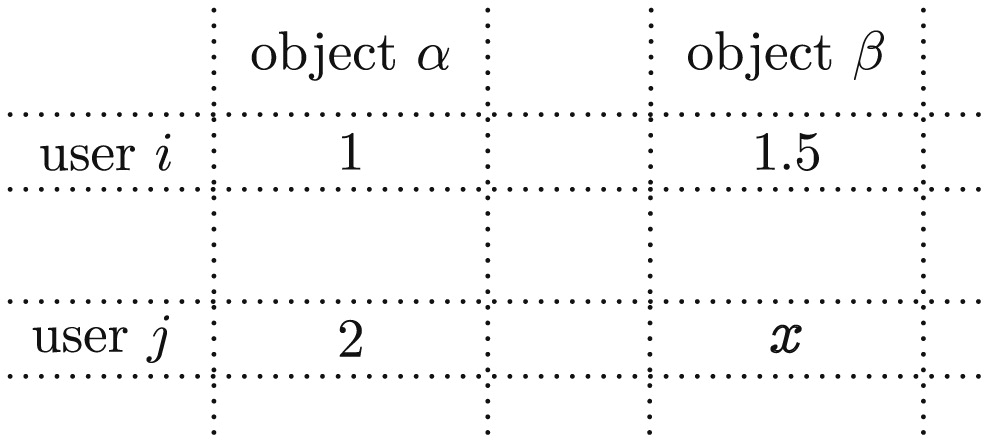
\includegraphics[width=0.75\textwidth]{./diagrams/slope one predictor.jpg}
	\caption{Slope One predictor. Adapted from \cite{LU20121}}
	\label{fig:fig3}
\end{figure}

\subsection{Memory-based}
Memory based algorithms can be divided into two categories:
user-based\cite{WANG2017102} and item-based algorithms.
\medskip

\subsubsection{User-based}
User-based Collaborative Filtering is among the most successful and widely implemented techniques in RS's. It recommends items to a target user based on opinions of other similar users to them . After forming the neighborhood, the new rating for the target user-item pair is estimated considering the weights of different neighbors. That is, the higher is the similarity of a user with the target user, the more impact their rating has on the estimation of the target user’s rating. The new rating for user \textit{u} and item \textit{i} is predicted as \textit{rui~} using: \cite{8550639}

% \begin{figure}[H]
%     \centering %%redo as a normal math formula (not enough time)
%     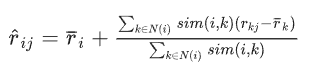
\includegraphics[width=0.5\textwidth]{./diagrams/math_formula.png}
%     \label{fig:fig3}
% \end{figure}
\begin{equation*} \mathop {\tilde {r}}\nolimits _{ui} =\frac {\sum \limits _{u'\in \mathop {NS}\nolimits _{u}} {(\mathop r\nolimits _{u'i})\times (\text {similarity}(\text {u},\text {u}'))}}{\sum \limits _{u'\in \mathop {NS}\nolimits _{u}} {\vert (\text {similarity}(\text {u},\text {u}'))\vert }}\tag{1}\end{equation*}

where NSu is the neighbor set of target user u with k members
% \cite{CHANG2025121355}
% add italics to specific letters for better understanding
% maybe replace it by something else because it is from a different source now

\subsubsection{Item-based}
When estimating an unknown rating value, first Eq. (1) is modified to calculate the Pearson correlation between items rather than users. Then, the new ratings are calculated using Eq. (2):
\begin{equation*} \mathop {\tilde {r}}\nolimits _{ui} =\frac {\sum \limits _{i'\in \mathop {NS}\nolimits _{i}} {(\mathop r\nolimits _{u{i}'})\times (\text {similarity}(\text {i},\text {i}'))}}{\sum \limits _{i'\in \mathop {NS}\nolimits _{i}} {\vert (\text {similarity}(\text {i},\text {i}'))\vert }}\tag{2}\end{equation*}
where \textit{NSi} is the neighborhood set of item \textit{i} \cite{8550639}

\section{Recommendation problems}

\subsection{Cold-start problem}
This refers to the challenge of making accurate recommendations while being limited by a small amount or lack of data available for new users,items or interactions. Without enough information , RS's struggle to create adequate suggestions .

\subsection{Scalability}
Due to vast amount of data, many algorithms without specific adjustments are not capable to sufficiently create recommendations and begin to experience performance issues

\subsection{Popularity Bias}
Due to RS's advising most popular products it tends to decrease sales and interest in smaller ones, potentially more suitable options for specific customers resulting in a bias towards the more mainstream options

%\newpage

\subsection{Solution}
There are many different types of recommendations that an RS can generate, and each of these types is appropriate in some and less appropriate in other conditions



\begin{figure}[H]
	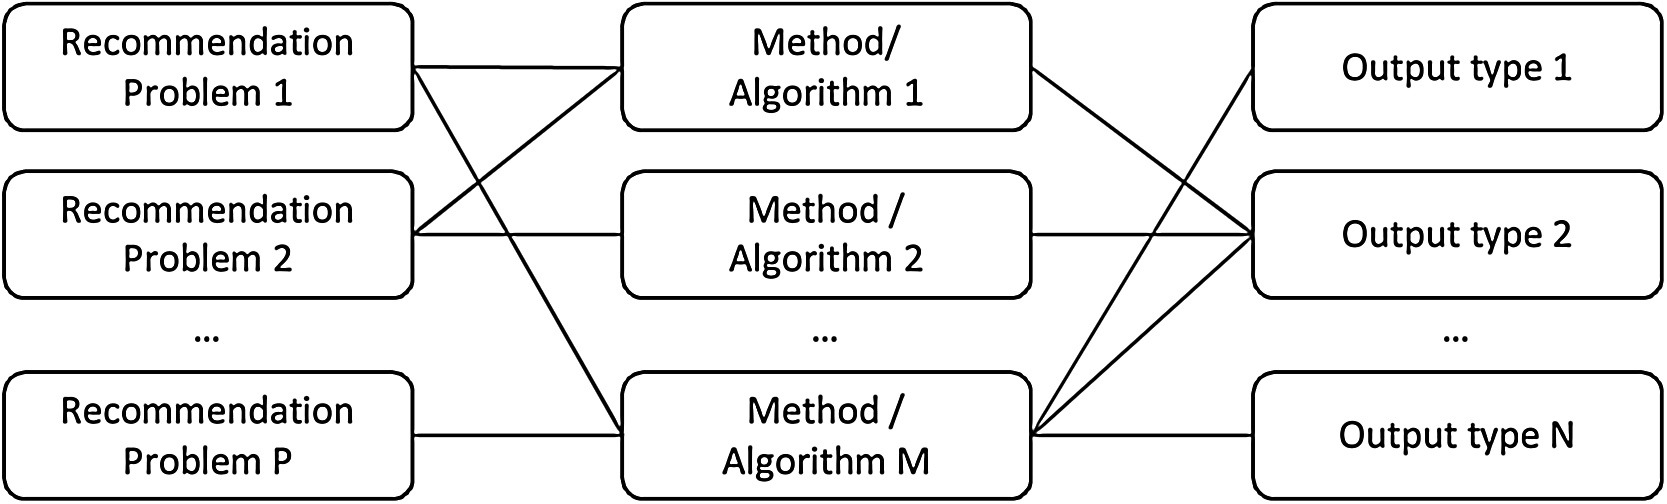
\includegraphics[width=1\textwidth]{./diagrams/recommendation_problems.jpg}
	\caption{Recommendation problems. Reproduced from \cite{GORGOGLIONE2019103143}}
	\label{fig:fig4}
\end{figure}

\section{Artificial intelligence usage}


\section{Efficiency of personalized ads}

\section{Discussion}

\section{Conclusion}


%\acknowledgement{Ak niekomu chcete poďakovať\ldots}


% týmto sa generuje zoznam literatúry z obsahu súboru literatura.bib podľa toho, na čo sa v článku odkazujete

\bibliographystyle{plain} % prípadne alpha, abbrv alebo hociktorý iný
\bibliography{literature}
\end{document}